\section{Introduction:}

Many useful algorithms are recursive in structure: to solve a given problem, they call themselves recursively one or more times to deal with closely related sub-problems. These algorithms typically follow a divide-and-conquer approach: they break the problem into several sub-problems that are similar to the original problem but smaller in size, solve the sub-problems recursively, and then combine these solutions to create a solution to the original problem.

\subsection{Analyzing Divide-and-Conquer Algorithms:}

When an algorithm contains a recursive call to itself, we can often describe its running time by a {\bfseries\itshape recurrence equation} or {\bfseries\itshape recurrence}, which describes the overall running time on a problem of size n in terms of the running time on smaller inputs. We can then use mathematical tools to solve the recurrence and provide bounds on the performance of the algorithm.

\begin{figure}[H]
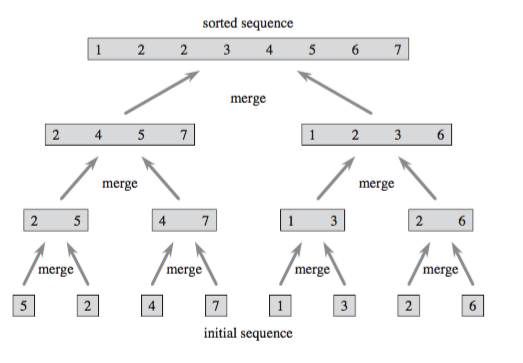
\includegraphics[scale=.6]{diagram.png}
\centering \linebreak \linebreak Figure 1.1.0: The operation of merge sort on the array A = { 5, 2, 4, 7, 1, 3, 2, 6 }. The lengths of the sorted sequences being merged increase as the algorithm progresses from bottom to top.
\end{figure}

A recurrence for the running time of a divide-and-conquer algorithm falls out from the three steps of the basic paradigm. As before, we let {\bfseries\itshape T ( n )} be the running time on a problem of size {\bfseries\itshape n}. If the problem size is small enough, say {\bfseries\itshape n $\leq$ c} for some constant {\bfseries\itshape c}, the straightforward solution takes constant time, which we write as $\theta ( 1 )$. Suppose that our division of the problem yields a subproblems, each of which is $\frac{1}{b}$ the size of the original. (For merge sort, both {\bfseries\itshape a} and {\bfseries\itshape b} are 2, but we shall see many divide-and-conquer algorithms in which {\bfseries\itshape a $\neq$ b}. It takes the time {\bfseries\itshape T ( $\frac{n}{b}$ )} to solve one subproblem of size $\frac{n}{b}$ , and so it takes time {\bfseries\itshape ( a ) ( T ( $\frac{n}{b}$ ) )} to solve {\bfseries\itshape a} of them. If we take {\bfseries\itshape D ( n )} time to divide the problem into subproblems and {\bfseries\itshape C ( n )} time to combine the solutions to the subproblems into the solution to the original problem, we get the recurrence: \hfill \break \break

\begin{ceqn}
\begin{align}
T( n ) = \left\{
\begin{array}{ll}
\theta ( 1 ) & \mathrm {if\ } n \leq c \\
aT(\frac{n}{b}) + D ( n ) + C ( n ) & \mathrm otherwise \\
\end{array}
\right.
\end{align}
\end{ceqn}

\pagebreak